\documentclass{article}
\usepackage[margin=.6in]{geometry}
\usepackage{parskip}
\usepackage{graphicx}
\usepackage{hyperref}
\hypersetup{
    colorlinks=true,
    linkcolor=black,
    urlcolor=red,
    linktoc=all
}

\title{Earth 121 Notes}
\author{}
\date{ }

\begin{document}

\maketitle

\tableofcontents


\section{Chapter 1 Introduction} % (fold)
\label{sec:chapter_1}
\subsection{The Science of Geology} % (fold)
\label{sub:the_science_of_geology}
Geo means earth and logos means discourse in greek which is where the name geology comes from. \textbf{Physical geology} examines composition of earth and \textbf{historical geology} looks for the origin of earth and its development. Most information about geology comes from \textbf{outcrops} where bedrock is exposed at the surface, but other times we dig down to get a good view.

\paragraph{Sir William Logan} was a geologist the only reason we care is that he's canadian and evidently we've got nothing better to be learning about.

Geology effects people when it results in natural disasters or resource shortages. On the flip side people can effect geology (blah blah pollution, deforestation, so on).

Historical view of the nature of earth:
\begin{itemize}
    \item \textbf{Catastophism} - created by James Ussher (crazy christian that said the earth was 4000), said that earth's landscape had been created by great catastrophes (things like mountains and valleys were created suddenly be a force that no longer operates)
    \item \textbf{Uniformitarianism} - created by James Hutton (scottish physician), says that the physical, chemical, and biologic laws that operate today operated in the geologic past so the stuff we see today have been shaping earth for a long time (small forces over a long time can make big changes)
\end{itemize}
% subsection the_science_of_geology (end)

\subsection{Geologic Time} % (fold)
\label{sub:geologic_time}
There was no good way to measure the age of earth until radioactivity was discovered. We now know its about \textbf{4.6 billion years old}. Before radio active dating we used \textbf{relative dating} which relied on finding the order of events without knowing their dates. This was done with \textbf{law of superposition} which states that in layers of sedimentary rocks or lava flows the youngest layer is at the top. It used fossils with the \textbf{priciple of fossil succession} which states that fossil organisms succeed one another in a definite and determinable order and any time span can be recognized by its fossil content (this is why the ages are not consistently long).

The earth is old so relative terms must be reevaluated to account for this when describing geology.
% subsection geologic_time (end)

\subsection{Early Evolution of Earth} % (fold)
\label{sub:early_evolution_of_earth}
 \paragraph{Planet}The universe began with the big bang, duh. The \textbf{nebular theory} suggests that the bodies of our solar system evolved fro an enormous rotating cloud called the solar nebula. 5 billion years ago the solar nebula (a cloud of hydrogen, helium, and heavier elements) collapsed due to gravity when it reached equilibrium it formed a \textbf{protosun}.

 \paragraph{Core} When gravitational collapse stopped things cooled down and elements with higher melting points started to condense to form clumps (this is why the core of planets is often nickel and iron). These clumps started to orbit and collide forming larger clumps, eventually becoming the four inner planets. During this time the temperature increased from all the collisions and got hot enough to melt dense blobs that sank to core making it liquid.

 \paragraph{Crust} This heating of the plant also resulted in chemical differentiation which allowed lighter elements to melt and float to the surface to form the crust(usually oxygen and oxygen seeking elements). Some heavier elements were carried up with the bubble of lighter elements resulting in gold, and uranium being near the surface.

\paragraph{Mantle} The heating of earth also created during the heating of earth so it became domibated by iron, magnesium, and oxygen seeking elements

\paragraph{Atmosphere} During the heating of earth gasses were allowed to escape which formed a primitive atmosphere which would be used by the first life forms.
% subsection early_evolution_of_earth (end)

\subsection{Plate Tectonics} % (fold)
\label{sub:plate_tectonics}
\textbf{Alfred Wegener} came up with the idea of \textbf{continental drift} (the idea that continents moved about the face of the planet) in the early twentieth century. The process that enables continental drift is called \textbf{plate tectonics}.

As world maps became more accurate we were able to see that certain continents fit together which was formalized by Wegener when he described \textbf{Pangaea}. This idea was first discounted because shorelines change continuously by erosion. When we look at the true outer boundary of continents, their \textbf{continental shelf} we can see where things fit together more concretely.

The biggest evidence of continental drift came from fossils of creatures that could not have crossed the ocean (namely a fern called Glossopteris) exiting in Africa and South America. It had large seeds that could not have blown far and no creature could carry it across. The plant also could only grow in certain climates but left fossils in locations they could never have grown.

We can see similar effects with mountain ranges (the Appalachians cross North America and fall off the edge beginning again under a different name in the British isles). These mountains are the same age and composition.

The last piece of evidence is the effects of past climates on the deposits in the area. Weathering in South America, Australia, and Africa shows the presence of past glaciers and coal deposits in North America and Europe show tropical climes in the past.
% subsection plate_tectonics (end)

\subsection{Planet of Shifting Plates} % (fold)
\label{sub:planet_of_shifting_plates}
The \textbf{lithosphere} consists of the uppermost part of the mantle is broken into plates that move about on convection currents in the mantle

Seven Plates:
\begin{itemize}
    \item North American
    \item South American
    \item Pacific
    \item African
    \item Eurasian
    \item Australian-Indian
    \item Antarctic
\end{itemize}
Some intermediary plates (Carribean, Nazca, Philippine, Arabian, Cocos, Juan de Fuca, and Scotia) and dozens of smaller ones have also been identified.

\paragraph{Divergent Boundaries} are boundaries where the plates move apart. This occurs mainly at a \textbf{mid-ocean ridge} but can also occur under rift valley son the continents. New material rises up to form new sea floor called \textbf{sea-floor spreading}. This results in that part of the plate becoming older, cooler, and thicker.

\paragraph{Convergent Boundaries} are boundaries where the plates move together causing the descent of oceanic lithosphere into the mantle, or the rise of continental margins (forming mountains). The leading edge of a converging plate is bent downwards to slide beneath the other in a \textbf{subduction zone}.

\paragraph{Transform Fault Boundaries} are boundaries where the plates slide past each other without forming or consuming lithosphere. These cause tones of earthquakes.
% subsection planet_of_shifting_plates (end)

\subsection{Earth's Internal Structure} % (fold)
\label{sub:earth_s_internal_structure}
Crust:
\begin{itemize}
    \item thin
    \begin{itemize}
         \item oceanic averages 7km
         \item continental averages 35km
     \end{itemize}
     \item oceanic is homogenious
     \item continental
     \begin{itemize}
         \item upper is similar granite
         \item lower is similar to basalt
     \end{itemize}
     \item continental density of $2.7 g/cm^3$
     \item continental is up to 4 billion years old
     \item oceanic density of $3.0 g/cm^3$
     \item oceanic less than 180 million years
\end{itemize}

Mantle:
\begin{itemize}
    \item 82\% of earths volume
    \item depth of 2900km
    \item mainly peridotite
    \item density $3.3g/cm^3$
\end{itemize}

Core:
\begin{itemize}
    \item mostly iron-nickle alloy
    \item extreme pressure
    \item density $11g/cm^3$
\end{itemize}

When you break up the earth based on physical properties you get five main layers.

\textbf{Lithosphere} is the outermost layer consisting of the crust and top of mantle that is cool and brittle.

\textbf{Asthenosphere} is the top layer of the mantle that is melty to allow the lithosphere to move about.

\textbf{Mesosphere} is a more rigid layer of the mantle than the asthenosphere, it still flow but much more slowly.

\textbf{Outer core} is the liquid layer that generates earth's magnetic field.

\textbf{Inner core} is the solid layer due to immense pressure.
% subsection earth_s_internal_structure (end)

\subsection{Earth's Spheres} % (fold)
\label{sub:earth_s_spheres}

\paragraph{Hydrosphere} is a dynamic mass of water cycling from sky to ocean and back. Covers 71\% of earth. This includes underground water and glaciers as well.

\paragraph{Atmosphere} is the gaseous envelope that surrounds earth.

\paragraph{Biosphere} is all life on earth.

\paragraph{Geosphere} is all the rocks and shit not in other spheres.

% subsection earth_s_spheres (end)

\subsection{The Face of Earth} % (fold)
\label{sub:the_face_of_earth}
The edge of a continent is the edge of its continental shelf, called \textbf{continental slope} which is the steel drop-off that extends from the outer edge of continental shelf to floor of deep ocean. There are two bands of young linear mountains, the cicum-Pacific belt (west americas and pacific island arcs) and the one that extends eastward from alps to himalayas. \textbf{Sheilds} are areas of continents that are relatively flat and composed of largely crystalline, granite-like rocks (some of the oldest rocks on earth are found there). The ocean basis containe the oceanic ridge system which si a 70 000km belt that winds around the globe consisting of layers of volcanic rock that have fractured and lifted. The ocean floor can also contain deep trenches
% subsection the_face_of_earth (end)

\subsection{Rock Cycle} % (fold)
\label{sub:rock_cycle}
The \textbf{rock cycle} is the process by which one type of rock changes into another.

\begin{enumerate}
    \item magma migrates upwards to crust where it cools and solidifies (called crystallization) resulting in \textbf{igneous rock}
    \item igneous rock is weathered into dust and moved around by gravity, water, glaciers, wind, or waves to be deposited as \textbf{sediment}, this undergoes lithification where it is compacted by the layers above it into \textbf{sedimentary rock}
    \item sedimentary rock is then barried deep in the earth and subjected to heat and pressure (from mountain building or magma) which turns it into \textbf{metamorphic rock}, this rock will eventually melt to complete the cycle
\end{enumerate}
% subsection rock_cycle (end)

% section chapter_1 (end)

\section{Ch 12 (272-277) : A Scientific Revolution Begins} % (fold)
\label{sec:ch_12_272_277_a_scientific_revolution_begins}
\subsection{Sea-floor Spreading Hypothesis} % (fold)
\label{sub:sea_floor_spreading_hypothesis}
Harry Hess came up with the theory of sea-floor spreading in the early 1960's. This was that ocean ridges are located above somes of upwelling in the mantle. This explained why rock from drilling into the ocean crust was all relatively young. He also explained that the sea floor was carried like a conveyer belt which would explain peices of the ocean floor that looked like they used to be islands. This proved that trenches are places where the crust is being consumed while it descends into the mantle.
% subsection sea_floor_spreading_hypothesis (end)

\subsection{Geomagnetic Reversals} % (fold)
\label{sub:geomagnetic_reversals}
A common occurrence is that the earth's magnetic field switches polarity, so rocks that are solidifying during that it will be magnetized opposite. \textbf{Normal polarity} is the direction of polarity of the current magnetic field and \textbf{reverse polarity} is the opposite. This was verified by examining lava flows from various ages. Scientists found trends of high and low intensity stripes of magnetism caused parallel to the ridge crest by using a \textbf{magnetometer} to measure magnetism of rocks. The alternate explanation (from Lawrence Morley) was that the high ridges were caused by normal polarity (rocks enhance the existing field) and low strips were formed during reverse polarity causing a weakening in the field there. Sea-floor spreading adds ocean floor at the middle of a stripe of magnetism maintaining the pattern as magnetism switches back and forth causing a mirror image to form on either side of the crack.
% subsection geomagnetic_reversals (end)

\subsection{Last Puzzle Piece} % (fold)
\label{sub:last_puzzle_piece}
Tuzo Wilson combined the theory of sea-floor spreading, the theory of tectonic plates, and the theory of types of plate boundaries, into the theory of tectonics.
% subsection last_puzzle_piece (end)
% section ch_12_272_277_a_scientific_revolution_begins (end)


\section{Chapter 2 Minerals} % (fold)
\label{sec:chapter_2}
\textbf{Minerals} are any naturally occurring inorganic (usually) solids that posess an orderly internal structure and a definite chemical composition. A \textbf{rock} is any solid mass of mineral that occurs naturally. Some rocks are only one mineral but most are aggregates. Some rocks have nonmineral matter like volcanic rocks that have classy substances and coal which has organic matter.

\subsection{Composition of Minerals} % (fold)
\label{sub:composition_of_minerals}
Earth has approximately 4660 minerals which are defined by their chemical composition and internal structure.

Atomic bonding happends due to interactions by valence electrons. An \textbf{ionic bond} is when one or more electrons are transferred between atoms. This creates an anion (negetively charged ion) and cation(positively charged ion). Ionic compounds consist of an orderly arrangement of oppositely charged ions assembled in a definite ratio to achieve net neutral charge. A \textbf{covalent bond} is when two atoms share electrons resulting in a bond stronger than ionic. Covalent bonds are more common.
% subsection composition_of_minerals (end)

\subsection{Structure of Minerals} % (fold)
\label{sub:structure_of_minerals}
The structure of ionic compounds is determined by the charges of the ions involved and their sizes. A positive ion will be surrounded by as many negative ions as it can while maintaining neutrality. Ex halite (table salt) forms cubes due to their orderly arrangement. \textbf{Polymorphs} are compounds that able to join in multiple geometries resulting in two minerals with same composition but different structures (ex graphite and diamonds). Polymorphs often happen due to temperature and pressure differences while they form.
% subsection structure_of_minerals (end)

\subsection{Physical Properties of Minerals} % (fold)
\label{sub:physical_properties_of_minerals}
\textbf{Crystal Habit} is the external expression of a mineral that reflects the orderly internal arrangement of atoms. Happens when a mineral forms without space restrictions, often crystals will compete for space resulting in a jumbled mess.

\textbf{Lustre} is the appearance or quality of light reflected from the surface of a mineral crystal. Lustre can be metallic  (like pyrite) or non-metalic (like quartz). Other adjectives are vitreous (glassy), pearly, silky, resinous, or earthy.

\textbf{Color} is not of good indicator of mineral type a small impurities in minerals can drastically change their color (for example amethyst is just impure quartz).

\textbf{Streak} is the color of a mineral in its powdered form. This is found by rubbing the mineral across unglazed porcelain called a streak. This is a better indicator than color is.

\textbf{Hardness} is the minerals resistance to abrasion or scratching. It is determined by rubbing the mineral against one of known hardness and using the \textbf{Mohs Scale} of relative harness. This is 10 minerals arranged from softest to hardest.

\textbf{Cleavage} is the tendency of a mineral to break along planes of weak bonding, defined by amount and angle. Minerals with cleavage have smooth surfaces. For example micas have weak bonds in only one direction to sthey form thin flat sheets. Some, like quartz have no cleavage (note: cleavage is not habit, cleavage is how it breaks not forms).

\textbf{Fracture} is how the mineral breaks aside from cleavage. For example quartz breaks smoothly like glass or seashells which is called a conchoidal fracture, other minerals splinter or fibre. Most minerals fracture unevenly.

\textbf{Specific gravity} is a number representing the ration of the weight of a mineral to the weight of an equal volume of water
% subsection physical_properties_of_minerals (end)

\subsection{Mineral Classes} % (fold)
\label{sub:mineral_classes}
Minerals that make up the earth's crust are classified as rock-forming minerals. The bulk of these are made of oxygen, silicon, aluminum, iron, calcium, sodium, potassium, and magnesium.
% subsection mineral_classes (end)

\subsection{Silicates} % (fold)
\label{sub:silicates}
These are formed by the combination of oxygen and silicon. This fundimental building block is called the \textbf{silicon-oxygen tetrahedron} which has four oxygen ions surrounding a silicon ion. The tetrahedron can  form single or double chains, or sheet structures by linking shared oxygen ions. Most common though is for the tetrahedron to become a jumbled 3D structure. We define these structures by their silicon to oxygen ratio. All of these structures have net negative charge so metal cations work as mortar to hold it together at the ends. You can swap out atoms that are about the same size without altering the mineral structure, this is denoted by parenthesis around an element list in the formula. The only anion available is oxygen so its always used, but silicon is the smallest of the cations so it bonds the strongest to it.
% subsection silicates (end)

\subsection{Common Silicate Minerals} % (fold)
\label{sub:common_silicate_minerals}
Feldspar (field-crystal) are the most common silicate minerals making up more than half the earths crust. Quartz is the second most common and only one made of pure silicon and oxygen. Silicates form when magma cools and solidifies. The enviroment when this happens determines what kind of silicate forms, this can be used to determine a minerals birth from inspection.

\textbf{Ferromagnesian Silicates}, sometimes called Dark Silicates, these are silicates containing iron or magnesium. The iron causes the silicate to be dark in color and have higher specific gravity.

Most common types:
\begin{itemize}
    \item olivine: high temperature silicate that is black or olive green, glassy, with conchoidal fracture
    \begin{itemize}
        \item part of mantle
        \item individual silica tetrahedra linked to iron causing no consistent places of weakness so no cleavage
        \item forms small rounded crystals
    \end{itemize}
    \item proxenes: complex minerals important part of dark igneous rocks, single chain
    \begin{itemize}
        \item most common is augite: dark, two cleavages meet at 90 degree, single chains bonded by iron, cleaves parallel to chain
    \end{itemize}
    \item amphibole, double chain:
    \begin{itemize}
        \item most common is hornblende: dark green to black, two cleavages meet at 60 and 90 degrees, double chain (wider chain means wider angle of cleavage),
    \end{itemize}
    \item biotite: iron rich member of mica group, silica sheet form, sheet cleavage, shiny black,
    \item garnet: forms equidimensional crystals, often dark brown or red
\end{itemize}

\textbf{Nonferromagnesian silicates}, sometimes called light silicates, have a specific gravity of 2.7 due to not containing iron or magnesium.

Most common types:
\begin{itemize}
    \item Muscovite: member of mica group, pearly, so thin its transparent (used for windows), very shiny
    \item Feldspar: most common mineral group, two cleavage at 90 degrees, about 6 on Mohs scale, glassy to pearly lustre
    \begin{itemize}
        \item orthoclase: type that contains potassium, light creme to pink, no striations
        \item plagioclase: type that contains sodium and calcium, white to grey to blue, has striations
    \end{itemize}
    \item Quarz: only silicon and oxygen, perfect 2-1 ratio means no metals needed, 3D framework, strong bonds make it hard, conchoidal fracture, colored by impurities
    \item Clay: has sheet structure (not a mica), fine grained only studied at microscopic level, from chemical weathering of other silicates so very common in soil
    \begin{itemize}
        \item kaolinite: most common, used in chinaware, and highgloss paper
    \end{itemize}
\end{itemize}

% subsection common_silicate_minerals (end)

\subsection{Nonsilicate Minerals} % (fold)
\label{sub:nonsilicate_minerals}
\paragraph{Carbonite} % (fold)
\label{par:carbonite}
A carbonate ion and cations. Calcite uses calcium and dolomite uses calacium-magnesium. These two are very similar, vitreous lustre, 3 hardness, rhobmic cleavage (three directions not at 90). You can tell them apart by dilute hydrochloric acid which dolomite reacts much more slowly to. These are often found in sedimentary rock limestone.
% paragraph carbonite (end)

\paragraph{Sedementary rocks} % (fold)
\label{par:sedementary_rocks}
Halite (salt), sylvite (fertilizer), and gypsum (plaster) are found in thick layers that used to be ancient seas.
% paragraph sedementary_rocks (end)
% subsection nonsilicate_minerals (end)

% section chapter_2 (end)


\section{Ch 5 (109-120)} % (fold)
\label{sec:ch_5_}
\subsection{Earth's External Processes} % (fold)
\label{sub:earth_s_external_processes}
\textbf{External processes} are ones that happen near the surface (like weathering and erosion) and \textbf{internal process} are ones that derive their energy from earth's interior (like volcanos and mountains)
% subsection earth_s_external_processes (end)

\subsection{Weathering} % (fold)
\label{sub:weathering}
\textbf{Mechanical weathering} is accomplished by physical forces that break rock into smaller eices without chaning its mineral compostion. \textbf{Chemical weathering} is a chemical transformation of rock into new compounds.
% subsection weathering (end)

\subsection{Mechincal Weathering} % (fold)
\label{sub:mechincal_weathering}
This is just breaking rock into smaller and smaller pieces, there are three main ways to do this.

\paragraph{Frost Wedging} % (fold)
\label{par:frost_wedging}
is when liquid water seeps into cracks in rock then expands due to freezing which breaks the rock apart. This happens alot in mountains and polar regions were freezing and thawing happen alot. When these loose rocks tumple into large piles they are called \textbf{talus slopes} which you see at the base of steep outcrops. This fucks up roads in Canada (salt makes it worse).
% paragraph frost_wedging (end)

\paragraph{Sheeting} % (fold)
\label{par:sheeting}
is when large masses of igneous rock are exposed by erosion causing concentric slabs to break loose making onion like layers. Weathering and erosion remove upper layers of rock decreasing the pressure on deeper igneous rock causing it to expand. More erosion makes these sheets flake of creating an \textbf{exfoliation dome}, When mining deep rocks have be known to explode due to released pressure.
% paragraph sheeting (end)

\paragraph{Biologic Activity} % (fold)
\label{par:biologic_activity}
causes weathering when plants dig deep with their roots, often breaking up rock in the process, and their seeds settle into cracks and break them apart as they grow. Moss can event enhance chemical breakdown from the surface. Burrowing animals break down rock by moving it to the surface and dead animals produce acids that break things down chemically.
% paragraph biologic_activity (end)
% subsection mechincal_weathering (end)

\subsection{Chemical Weathering} % (fold)
\label{sub:chemical_weathering}
Rocks decompose into elements that are stable in the environment, so if the rock's environment is stable chemical weathering doesn't happen. Water itself is a good solvent, but it can carry materials that speed up that process. There are three main processes.

\paragraph{Dissolution} % (fold)
\label{par:dissolution}
is the breakdown of materials that dissolve in water. This is due to the polar nature of water. Halite is a good example where the polarity of water disrupts the net neutral charge of the ions involved releasing the ions into water. Most minerals don't dissolve in pure water, but most water contains small amounts of acid that increase the corosive force of water. Once example is carbonic acid which forms when $CO_2$ dissolves into rain drops. Calcite (limestone and marbel) is very susceptible to acid rain. The calcium carbonate in it is broken into calcium ions and bicarbonate. This forms the limestone caverns all over north america. This also bleeds calcium ions into the ground water making hard water that reacts with soap to become insoluble (can add a softener).
% paragraph dissolution (end)

\paragraph{Oxidation} % (fold)
\label{par:oxidation}
is when iron rich minerals rust due to electrons being lost from one element during the reaction with oxygen.  This forms hematite or limonite which gives iron rich minerals their dark coloration. The iron must first been freed from the silicate structure for this to happen (the process is called hydrolysis). Other silicates without iron can suffer from oxidation (pyrite breaks down into sulphuric acid and iron oxide) which can cause environmental issues. This is called mine acid because mining exposes the minerals to the moisture needed to form the acid.
% paragraph oxidation (end)

\paragraph{Hydrolysis} % (fold)
\label{par:hydrolysis}
is the reaction of any substance with water. Ideally this is pure water but often it contains ions. This is the process that breaks down feldspar into clay resulting in is popularity in soil. In this the hydrogen ions in water replace the potassium ions breaking up the crystal structure and making the potassium available for plants to use. This also creates some silica that is carried to the ocean for critters to make their shells with. Clay minerals are very stable so they are usually the result of chemical weathering which makes them so common. Quartz is very resistant to chemical weathering.
% paragraph hydrolysis (end)

\paragraph{Alerations Caused by Chemical Weathering} % (fold)
\label{par:alerations_caused_by_chemical_weathering}
Chemical weathering attacks corners and outcrops more readily due to their increased surface area causing rounded rocks in a process called \textbf{spheroidal weathering}.
% paragraph alerations_caused_by_chemical_weathering (end)

\subsection{Rates of Weathering} % (fold)
\label{sub:rates_of_weathering}
Weathering can be sped up by a number of factors:
\begin{itemize}
    \item surface area
    \item rock composition (order of silicate mineral weathering is same as order of crystalization)
    \item climate (temperature and moisture effect chemicals present and vegetation)
    \item attributes of near by rocks (called \textbf{differential weathering})
\end{itemize}
% subsection rates_of_weathering (end)

% subsection chemical_weathering (end)

% section ch_5_ (end)

\section{Ch 3: Igneous Rocks} % (fold)
\label{sec:ch_3_igneous_rocks}
\subsection{Magma} % (fold)
\label{sub:magma}
Igneous rocks form when magma cools and solidifies. Magma is formed through a process called \textbf{partial melting} which occurs at various levels within the earth's crust. A body of magma rises towards the surface due to its lower density. If magma reaches the earth's surface it becomes \textbf{lava}, which happens through a volcanic eruption. Igneous rock that forms when magma solidifies at the surface is called \textbf{extrusive/volcanic}. If magma doesn't reach the surface and crystallizes at dept the rock that forms is called \textbf{intrusive/plutonic}. Bodies of this rock are called plutons which are only exposed when the crust is uplifted.

\paragraph{Formation of Magma} % (fold)
\label{par:formation_of_magma}
Most magma originates in mantle causing most igneous rock to be at divergent plate boundaries. Lots of magma is also created at subduction zones. Some magma is even made in the earth's mantle due to temperature and pressure. The temperature increases by about $25^{\circ} C$ per kilometer down called the \textbf{geothermal gradient}. At the edge of the crust and mantle rocks are super hot but still solid so any heat that is added will form magma (like at subduction zones with friction, or sinking at subduction points or rising up). Pressure also increases with depth raising the melting point for deeper rocks. When confining pressure drops enough \textbf{decompression melting} occurs (usually divergent boundaries). Water and gasses called \textbf{volatiles} can lower the melting point of rock. This happens at oceanic subduction zones where water seeps into the wedge.
% paragraph formation_of_magma (end)

\paragraph{Nature of Magma} % (fold)
\label{par:nature_of_magma}
The liquid portion of magma is called \textbf{melt} and is made of mobile ions of silicon, oxygen, and lesser amounts of common metals. The solid portion are just bits that have already crystalized from the melt. Magma often has water, carbon dioxide, and sulphur dioxide volatiles in it. Volatiles stay dissolved due to pressure until the magma cools enough to crystallize and let them escape.
% paragraph nature_of_magma (end)

\paragraph{Crystaline Rock} % (fold)
\label{par:crystaline_rock}
As magma cools its ions lose their mobility and arrange themselves into crystalline structures in a process called \textbf{crystalization}. Generally the silicon and oxygen atoms goind fist into tetrahedra which then join into embryonic crystal nuclei. Earlier crystals have more space to grow in and so develop better. This process is much more complicated due to temperature ranges .
% paragraph crystaline_rock (end)

% subsection magma (end)
\subsection{How Magma Evolves} % (fold)
\label{sub:how_magma_evolves}
There are different kinds of lavas, sometimes from the same volcano.

\paragraph{Bowen's Reaction Series} % (fold)
\label{par:bowen_s_reaction_series}
Magma crystalizes at a large range of temperatures so Bowen tested this in laboratory conditions. He found that minerals crystalize in a fashion relative to their melting points. Throughout this process the temperature and composition of the melt will alter. At about one third cooled the magma will be completely drained of fe, mg, and ca because those materials are used in the formation of the earliest melting compounds. This leaves the magma silica rich, it has evolved. There are many ways for magma to evolve.

\textbf{Crystal setting} is when earlier formed minerals sink as they are denser than the melt. The remaining melt will solidify into a very different rock from its parent magma called \textbf{magmatic differentiation}. If the solid crystals remain in contact with the melt they will evolved into the next mineral in the sequence called \textbf{Bowen's reaction series}. Minerals that form in the same temperature range in Bowen's series  are found together in the same igenous rock.

As magma moves about it pulls in surrounding host rock in a process called \textbf{assimilation}. This happens when magma is moving up near the surface where rocks are brittle. The upward force of the magma causes cracks that can dislodge blocks of rock to mix into the magma. It can also happen deep down where the magma is hot enough to melt the surrounding rock.

Multiple magma bodies can intrude on each other which is called \textbf{magma mixing}. Convective flow mixes the magmas into a fluid of intermediate composition

% paragraph bowen_s_reaction_series (end)

\paragraph{Partial Melting} % (fold)
\label{par:partial_melting}
Magma evolution also happens during melting, much the same way as it happens during cooling. If melting is complete the magma composition will resemble the rock it came from, but often melting is not complete. This results in melt that is enriched in ions from minerals with the lowest melting temperatures and a bunch of unmelted crystals.

Mafic magmas originate from the melting of peridotite (main thing in the upper mantle). When mafic magmas result for melting of mantle rock they are called primary magmas since they haven't evolved. Mafic magma often migrates upwards eventually erupting out.

Intermediate magmas  and felsic magmas are found only at continental margins because they are the result of interactions between mafic magmas and silica rick components of the crust. Inbetween felsic and mafic magmas are \textbf{andiesitic composition} magmas. This can also form during magmatic differentiation of mafic magma which is why they are sometimes called secondary magmas. Felsic rocks are too common to be the result of differentiation of intermediary magma so they are likely the end product of cyrstallization of intermediate magma or the result of partial metlting of silica rich rock. Felsic magma is much thicker so doesnt erupt and forms large plutonic bodies.
% paragraph partial_melting (end)

% subsection how_magma_evolves (end)


\subsection{Igenous Compositions} % (fold)
\label{sub:igenous_compositions}
\paragraph{Felsic VS Mafic} % (fold)
\label{par:felsic_vs_mafic}
Most igneous rock can be divided into two groups based on the proportions of light and dark minerals. Igneous rocks dominant in light minerals (less than 10\% dark) are called felsic. These are rich in silica and make up most of the crust. Since granite is the most common they are often referred to as having a granitic composition. Rocks that are dominated by dark minerals are called mafic. These are sometimes said to have basaltic compositions because basalt is the most common. Mafic rocks make up most of the ocean floor.
% paragraph felsic_vs_mafic (end)

\paragraph{Other Groups} % (fold)
\label{par:other_groups}
Rocks between felsic and mafic (at leas 25 \% dark) are called intermediate or andesitic composition. Rocks that are almost entirely dark minerals are called \textbf{ultramafic}. These are rare at the surface.
% paragraph other_groups (end)

\paragraph{Silica Content} % (fold)
\label{par:silica_content}
Silica content is inversly related to the metal content in a mineral. Silica increases the viscousness of the magma. Silica also decreases the melting temperatures.
% paragraph silica_content (end)

% subsection igenous_compositions (end)

\subsection{Igneous Texture} % (fold)
\label{sub:igneous_texture}
\textbf{Texture} is the overall appearance of a rock based on the size, shape and arragement of crystals.

\paragraph{Crystal Size} % (fold)
\label{par:crystal_size}
If magma cools slowly it forms larger but fewer crystals. If magma cools too quickly and results in rocks that consist of unordered ions it is called \textbf{glass}.
% paragraph crystal_size (end)

\paragraph{Types of Textures} % (fold)
\label{par:types_of_textures}


\textbf{Aphanitic} texture is used to describe rocks that form at the surface with rapid cooling resulting in a very fine grained texture. The crystals in them are so small that you need a microscope to tell them apart. This makes mineral identification impossible so they are characterized by color (light, medium, dark). These rocks often have cas bubbles where the lava solidified fast enough to catch gas, these are rocks are called \textbf{veicular texture}.

\textbf{Phaneritic} texture is used to describe rocks that form when large masses of magma cool slowly far below the surface resulting in a coarse grained texture. The crystals in these rocks can be identified by magnifying glass.

\textbf{Porphyritic} texture is used to describe rocks that have very large crystals in them as a result of deep magma growing crystals then suddenly changing environments. These rocks have large crystals, called \textbf{phenocrysts}, embeded in a matrix of smaller crystals called, \textbf{groundmass}.

\textbf{Glassy} texture is used to describe when molten rock is extruded into water or the air causing it to cool very rapidly resulting in unordered ions (no crystals formed). This can also happen when magma is very viscous (high in silica).

\textbf{Pyroclastic} texture is used to describe when igneous rock is formed from the consolidation of rock fragments. This is also sometimes called \textbf{fragmental texture}.

\textbf{Pegmatitic} texture is used to describe when rocks are composed of only large crystals called \textbf{pegmatites}. These are usually found on the edges of plutons. These form during the late stages of crystallization when there are lots of volatiles that enhance ion migration to speed up crystal formation. This is how the large number of large crystals exist.
% paragraph types_of_textures (end)
% subsection igneous_texture (end)


\subsection{Naming Igneous Rocks} % (fold)
\label{sub:naming_igneous_rocks}
Igneous rocks are classified by their mineral composition and texture.

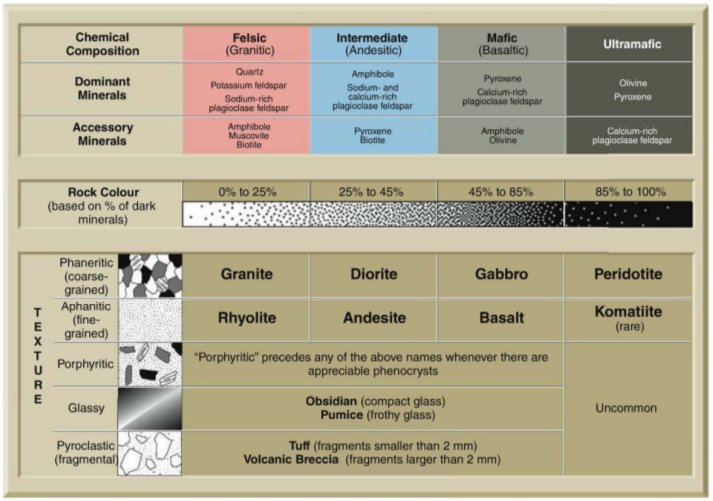
\includegraphics[width=7in]{igneous-classes}

\subsubsection{Felsic(Granitic)} % (fold)
\label{subsub:felsic}

\textbf{Granite}:
\begin{itemize}
    \item is the most well known due to its beauty and abundance.
    \item 20 \% quartz, 65\% feldspar (sodium and potassium rich)
    \begin{itemize}
        \item quartz crystals irregular shape, glassy clear-grey color
        \item feldspar crystals less glassy, grey-salmon color, rectangular shape
    \end{itemize}
    \item can be porphyric texture (speckled) with feldspar crystals $<$ 1cm
    \item by product of mountain building, resistant to weathering so gets left as a core
    \item granite also used to describe any rock that is intrusive coarse grained
    \item often found in large plutonic masses
\end{itemize}

\textbf{Rhyolite}:
\begin{itemize}
    \item extrusive equivalent of granite
    \item full of light silicates (usually light grey or pink in color)
    \item aphanitic
    \item often contains glass or voids due to rapid cooling on surface
    \item if phenocrysts they are small (quartz or potassium feldspar)
\end{itemize}

\textbf{Obsidian}:
\begin{itemize}
    \item dark, glassy
    \item formed when silica rich laval is quenched quickly
    \item unordered ions, due to quick cooling
    \item high silica concentration (despite dark color)
    \item excellent conchoidal fracture so it holds sharpness well
\end{itemize}

\textbf{Pumice}:
\begin{itemize}
    \item forthy texture
    \item forms when large amounts of gass escape through lava (found near obsidian a lot)
    \item large number of voids
    \item sometimes will float
    \item flow lines can indicate movement during cooling
\end{itemize}
% subsubsection felsic (end)

\subsubsection{Intermediate} % (fold)
\label{subsub:intermediate}
\textbf{Andesite}:
\begin{itemize}
    \item medium grey
    \item fine grained
    \item name comes from Andes mountains where they are commonly found
    \item often has porphyritic texture
    \item if porphyritic pyrocysts are light, rectangular, plagioclase feldspar, or black, elongate amphibole crystals
    \item often looks like rhyolite
    \item very small amounts of quartz
\end{itemize}

\textbf{Diorite}:
\begin{itemize}
    \item plutonic version of andesite
    \item coarse grained
    \item intrusive
    \item no visible quartz crystals
    \item high percentage of dark silicate minerals
    \item mostly sodium-calcium plagioclase felsdpar and amphibole giving it a salt and pepper look
\end{itemize}

% subsubsection intermediate (end)


\subsubsection{Mafic(basaltic) and Ultramafic} % (fold)
\label{subsub:mafic_and_ultramafic}
\textbf{Basalt}:
\begin{itemize}
    \item very dark green-black
    \item mostly pyroxene and calcium plagiuclase feldspar with some olivine and amphibole
    \item contains light colored feldspar phenocrusts or glassly olvine phenocrysts
    \item most common extrusive igenous
    \item many volcanic islands and upper layers of oceanic crust are basalt
\end{itemize}

\textbf{Gabbro}:
\begin{itemize}
    \item intrusive equivalent of basalt
    \item dark green to black
    \item proxyene and calcium rich plagioclase feldspar
    \item makes up lots of oceanic crust
\end{itemize}

\textbf{Peridotite}:
\begin{itemize}
    \item most of the upper mantle is peridotite
    \item ultramafic
    \item olivine, proxene and calcium-rich plagioclase feldspar
    \item very rare, only make it to serfice as slivers in mountain building
\end{itemize}
% subsubsection mafic_and_ultramafic (end)

\subsubsection{Pyrocastic Rocks} % (fold)
\label{subsub:pyrocastic_rocks}
\textbf{Tuff} is most common pyrocastic rock and is composed of tiny ash-sized fragments that become cemented together. If these particles remain hot enough to fuse it is called \textbf{welded tuff}, which is mostly small glass shards with bits of pumice and other rock fragments. These are very common is volcanic areas. They formed millions of years ago when ash from volcanoes moved like avalanches. If the pyrocastic rocks are make of partivles alrger than ashe they are called colanic breccia and consist of streamlined fragments that solidified in air, or blocks broken from the walls of the volcanic vent.
% subsubsection pyrocastic_rocks (end)

% subsection naming_igneous_rocks (end)

\subsection{Intrusive Igneous Bodies} % (fold)
\label{sub:intrusive_igneous_bodies}
\paragraph{Nature of Plutons} % (fold)
\label{par:nature_of_plutons}
Plutons occur when magma solidifies at depth. Plutons are classified according to shape as either \textbf{tablular} or \textbf{massive} and classified by their orientation relative to host rock. \textbf{Discordant} rocks are cut across existing rock and \textbf{concordant} rocks form parallel to sedimentary layers. The largest plutons are remnants of magma chambers that fed old volcanoes.
% paragraph nature_of_plutons (end)

\paragraph{Dykes} % (fold)
\label{par:dykes}
are tabular, discordant plutons formed when magma is injected into fractures. These are commonly found in groups with a non-observable parent pluton. Sometimes the force of the magma rising is enough to cause the cracks that the dyke eventually filled.
% paragraph dykes (end)
\paragraph{Sills} % (fold)
\label{par:sills}
are tabular concordant plutons which form when magma is injected along sedimentary bedding surfaces. Horizontal sills are the most common but they can occur at any orientation so long as there is sedimentary rock with that orientation. Sills tend to be the product of fluid mafic magmas in shallow environments. Sills often display \textbf{columnar joints} which form as igneous rocks cool and develop shrinkage fractures that produce elongate pillars which often gets sills confused for buried lava flows. The difference between sills and lava flows is that lava flows often have voids in their upper layers from gas escaping while sills often have particles of overlying rocks since they are forced in.
% paragraph sills (end)

% subsection intrusive_igneous_bodies (end)

\subsection{Laccoliths} % (fold)
\label{sub:laccoliths}
\textbf{Laccoliths} are formed when viscous magma seeps between sedimentary layers resulting in blister-like masses that arch the overlying strata upward into domes that can sometimes be seen on the surface.
% subsection laccoliths (end)

\subsection{Batholiths} % (fold)
\label{sub:batholiths}
\textbf{Batholiths} are the larges intrusive igneous bodies which occur in groups that form massive belts. A plutonic body must have a surface exposure greater than 100 square kilometers to be called a batholith, else it is called a \textbf{stock}. Batholiths are usually mad of felisic to intermediate rocks. Some are the joining of multiple plutons. Some mountain cores are batholiths that get exposed by weathering and uplifting.

\paragraph{Emplacement} % (fold)
\label{par:emplacement}
Large granitic batholiths can form withing sedimentary and metamorphic rock with little deformation which confused scientists. They could not see how the magma body made it through several kilometers of solid rock or where the displaced rock went. At great depths magma is so boyant it can push aside solid rock to move upward and the rock that is pushed aside slides in behind it. The body may break up rocks above it and melt the peices changing its own composition, but eventually it cools enough to stop moving. Evidence for magma moving through solid rock is found in peices of unmelted host rock found in the pluton after is is exhumed by erosion called \textbf{xenoliths}.

% paragraph emplacement (end)
% subsection batholiths (end)
% section ch_3_igneous_rocks (end)

\section{Chapter 4: Volcanoes} % (fold)
\label{sec:chapter_4_volcanoes}
\subsection{The Nature of Volcanic Eruptions} % (fold)
\label{sub:the_nature_of_volcanic_eruptions}
The primary features that effect a volcano's behavior is the magnas composition, temperature, and the amount of dissolved gases it contains. Most of those factors effect the magma's viscosity.

\paragraph{Viscosity} % (fold)
\label{par:viscosity}
is directly proportional to the magma's silica content. This is due to silica structures linking together into long chains. So felsic lavas are much slower than mafic lavals.
% paragraph viscosity (end)

\paragraph{Dissolved Gasses} % (fold)
\label{par:dissolved_gasses}
tend to decrease the viscosity and can even provide enough force during their escape to propel magma up through a \textbf{vent} or \textbf{conduit}. Before a volcano errupt its summit swells due to gases accumulating at the top. During an erruption the sudden decrease in pressure allows the gass to be released quickly. If the magma is mafic it can be propelled upward into a fountain. If the magma is feslic the gas expels jets of hot ash into buoyant plumes called \textbf{eruption columns}. Before this happens there is lots of differentiation letting iron rich crystals settle out leaving the upper part rich in silica and gases. This is how the gas contains small bits of ash due to little bits of magma being carried. Often the release of pressure allows lower layers of magma to build and erupt as well resulting in erruptions being a series of explosions. AFter the erruption phase is done the remaining de-gassed magma migrates upward slowly, There may be more gas build up after the initial eruption allowing more sporatic eruptions to happen.
% paragraph dissolved_gasses (end)
% subsection the_nature_of_volcanic_eruptions (end)

\subsection{Materials Extruded Duraing Eruption} % (fold)
\label{sub:materials_extruded_duraing_eruption}
\paragraph{Lava Flows} % (fold)
\label{par:lava_flows}
Hot mafic lava is very fluid allowing it to flow in thin broad sheets or thin ribbons. These can move as fast as a walking person (some have been clocked at 30km/h). This lava forms a skin like surface that wrinkles as it flows and are called \textbf{pahoehoe flows} (named in Hawaii where they are common). When lots of gas escape from the surface of the flowing lava it results in surface voids and a sharp jagged flow called \textbf{aa flow}. This flow continues to break as it goes making it look like an advancing mass of rubble. When lava flows into the ocean, or originates in it the lava quickly forms an hardened skin due to the cooling nature of water. The rest of the lava usually cannot break through this skin resulting in round spherical shapes called \textbf{pillow lavas}. Often lava drains out of the tunnels it used to escape when pressure is not enough to push it through resulting in \textbf{lava tubes}. These allo fluid lavals to move great distances from their source
% paragraph lava_flows (end)

\paragraph{Gasses} % (fold)
\label{par:gasses}
Volcanoes can emit so much gas that it effects the composition of the atmosphere. Gasses are also resposible for creating the passabeway that connects the magma chamber to the surface. The buoyant force of the rising magma makes cracks, but it is escaping gases that widen these cracks
% paragraph gasses (end)

\paragraph{Pyroclastic Materials} % (fold)
\label{par:pyroclastic_materials}
Often volcanoes spit out little particles that can land near the mouth making that cone shape you see, or can be carried very far away. The little ash particles are formed when the gas disolved in the magma starts to rapidly expand creating a froth which is blown into the air to rapidly cool in to tiny flassy fragments which often fuse to become welded tuff. Particles that are nut sized ar called \textbf{lapilli} or \textbf{cinders}. Larger particles are called \textbf{blocks} if they are hardened or \textbf{bombs} if not. Bombs are often elongated because they cool as they fly through the air.\textbf{Scoria} is pyroclastic material that contains voids from mafic magma.
% paragraph pyroclastic_materials (end)

 \paragraph{Nuee Ardente} % (fold)
 \label{par:nuee_ardente}
 \textbf{Pyroclastic flows} are flows that consits of hot gases infused with incandescent ash and larger rocks. The most destructive of these are \textbf{nuees ardentes} as they can race down steep slopes at 100km/h to wipe out whole towns. The ground facing portion of the flow is rich in particles and suspended by buoyant jets of gas escaping. The flow moves quick enough to overtake air and trap it below heating it to provide buoyancy allowing the flow to move unhindered by friction and contain large rock fragments. They form from the collapse of eruption columns.
 % paragraph nuee_ardente (end)

 \paragraph{Lahars} % (fold)
 \label{par:lahars}
 Steep sided volcanos can cause mudflows called lahars when volcanic debri becomes saturated with water to move rapidly down the slope. These can be triggered when large amounts of snow are melted by an eruption or even when there is heavy rain on volcanic deposites (volcano doesnt need to be erupting).
 % paragraph lahars (end)

% subsection materials_extruded_duraing_eruption (end)

\subsection{Volcanic Structures and Eruptive Styles} % (fold)
\label{sub:volcanic_structures_and_eruptive_styles}

\paragraph{Anatomy} % (fold)
\label{par:anatomy}
The central conduit for lava is called the \textbf{pipe} which terminates in a vent. A volcano is built up through successive eruptions and coolings of lava. There is a small depression at the top of the vent called the \textbf{crater} which are built up as ejected fragments collect around the vent. Some volcanoes can have multiple craters or a single large one called a \textbf{caldera}. Side tunnels off the pipe can form and ejected materials form parasitic cones on the side of the volcano. When side vents only emit gas they are called \textbf{fumaroles}.
% paragraph anatomy (end)

\paragraph{Shield Volcanoes} % (fold)
\label{par:shield_volcanoes}
These are volcanoes that form from the accumulation of fluid mafic lava resulting in broad domed structures (they look like a warrior's shield). Many grown up from the ocean floor to form islands. These have very large deep calderas that form when the roof of the volcano collapses, As they mature their magma thickens and eruptions become less frequent.
% paragraph shield_volcanoes (end)

\paragraph{Cinder Cones} % (fold)
\label{par:cinder_cones}
These are ejected lava fragments that harden while in flight as a product of gas rich mafic magma. Occassionally these are made of ash and pumice if the magma is silica rich. They have a very regular shape that is formed due to gravity. They are sloped with a crater on one end and elongated on the uphill side. Cinder cones usually form as a result of the last eruption of a volcano after which it solidifies its pipe. Cinder cones are usually 30-300 meters in height.
% paragraph cinder_cones (end)

\paragraph{Composite Volcanoes} % (fold)
\label{par:composite_volcanoes}
These are the pretties and deadliest volcanoes. Usually only found on the ring of fire. These are symetrical structures composed of lava and pyroclastic deposits as a product of gas rich magma having andesitic composition. These magmas are thick and travel short distances but also have explosive erruptions that spew great quantities. Composite volcanoes have very steep summit and gradually sloping sides due to larger pyroclastic ejecta gathering around the summit while smaller ejecta cover a larger area. In its early life lavas are more abundant and flow farther than latter on in life, also contributing to steep summit and sloping sides.

Huge mounds of volcanic debri around many cones can imply that a composite volcano had a massive landlist. Horseshoe shaped depression in summit imply an explosive eruption or landslide leaving a hole on one side of the summit.
% paragraph composite_volcanoes (end)


\paragraph{Calderas} % (fold)
\label{par:calderas}
These are collapsed depressions 1-10km in diameter firmed by the collapse of a large composite volcano summit followed by an explosion of pumice and ash, or the collapse of the top of a volcano caused by subteranian drainage, or the collpase of a large area without volcanic effect.
% paragraph calderas (end)

\paragraph{Fissure Eruptions and Lava Plateaus} % (fold)
\label{par:fissure_eruptions_and_lava_plateaus}
Fissures are cracks in the earth's crust allowing volcanic material through. Fissures can have many eruptions and this can lead to build up of basalt growing to thousands of meters in thickness. The lava escaping is very fluid allowing it to flow in sheets over great distances. \textbf{Flood basalt} is used to describe flows covering massive areas.
% paragraph fissure_eruptions_and_lava_plateaus (end)

\paragraph{Lava Domes} % (fold)
\label{par:lava_domes}
These are formed by maafic lavas that are squeezed out of the vent but dont really go anywhere resulting in a steep sided dome of congealed lava. Usually only the late stages of a mature, mainly andesitic composite volcano forms lava domes.
% paragraph lava_domes (end)

\paragraph{Volcanic Pipes and Necks} % (fold)
\label{par:volcanic_pipes_and_necks}
Pipes are the conduits through which volcanoes are fed magma. Ultramafic magmas as migrate up through pipes so quickly they form prisine samples of the mantle giving deep pipes the nickname of ``windows''. These also often have diamonds and other high preassure minerals in them.
% paragraph volcanic_pipes_and_necks (end)
% subsection volcanic_structures_and_eruptive_styles (end)

% section chapter_4_volcanoes (end)

\newpage
MIDTERM 1
\newpage
\section{Chapter 6: Sedimentary Rocks} % (fold)
\label{sec:chapter_6_sedimentary_rocks}
\subsection{What is a Sedimentary Rock} % (fold)
\label{sub:what_is_a_sedimentary_rock}
Sedimentary rocks are formed from the raw materials produced by weathering. This sediment is diposited by settinling out of fluid or air. These piles of sediment accumulate until the layers near the bottle are compacted by pressure into rocks. While sedimentary rocks only make up about 5\% of the crust they make up 75\% of the outcrops we see. Because sedimentary rocks are only found near the surface we can use their layers to learn about past environments on the surface. This is often where fossils are found.
% subsection what_is_a_sedimentary_rock (end)

\subsection{Turning Sediment to Rock} % (fold)
\label{sub:turning_sediment_to_rock}
\textbf{Diagenesis} is the term for all of the changes that take place after sediments are deposited and before they become metamorphic rock. Diagenesis occurs in the upper portion of the earth's crust at about 150-200 degrees Celsius. At 200 degrees it starts metamorphism. One process in diagenesis is \textbf{re-crystalization} where more stable minerals are formed from less stable ones. Another is \textbf{lithification} where unconsolidated sediments are transformed into solid rocks by compaction and cementation.

\paragraph{Compaction} % (fold)
\label{par:compaction}
This is the process where the weir of overlying material compresses the deeper layers. The deeper down, the more compacted sediment is. Compaction causes grains of sediment to get much closer together decreasing their \textbf{pore-space} and causes them to lose fluids. Due to this a significant percentage of volume is lost. The coarser the grain the less likely compaction will occur.
% paragraph compaction (end)

\paragraph{Cementation} % (fold)
\label{par:cementation}
This is a chemical process through which dissolved minerals preciptate through grains of sediment to fill the pore space and join the grains.
There are three main cementing materials with easy detection:
\begin{itemize}
    \item calcite: bubbles when hydrochloric acid is introduced
    \item silica: forms hardest rocks
    \item iron oxide: has red orange color
\end{itemize}

Some sedimentary rocks start as masses of interlocking crystals rather than as sediment.
% paragraph cementation (end)
% subsection turning_sediment_to_rock (end)
\subsection{Environments} % (fold)
\label{sub:environments}
\paragraph{Continental Environments} % (fold)
 \label{par:continental_environments}
 These are dominated by erosion and movement caused by streams. Sometimes glaciers and winds are more common. Glaciers often result in a poorly sorted mix of particles picked up from all over that are deposited by the glacier's melting water resulting in straified, sorted accumulations. Streams work by eroding and carying sediment as they go. This agitates the existing sediment allowing it to sort as it resettles (heaviest at the bottom). This is why very turbulent waters have lots of pebbles and larger grained rocks in their sediment and calmer waters have finer grains. At places where waters change speed you get large sediment build ups. For example at the bottom of a mountain stream you get a aluvial fan. You also form plains of sediment where floods are periodic forming floodplains. Where wind dominates you get aelian deposits that are well sorted as wind can lift small grains quite high.
 % paragraph continental_environments (end)

 \paragraph{Transitional Environments} % (fold)
 \label{par:transitional_environments}
 These are characterized by low gradients or quiet waters where fine grained sediment may be deposited under shallow water or exposed to air. This results in tidal flats. At the other end we have shorelines with violent wave and current action to form a beach. Most deltas are a result of transitional environments as rivers experience a sudden drop in speed making them drop their load.
 % paragraph transitional_environments (end)

\paragraph{Marine Environments} % (fold)
\label{par:marine_environments}
We divide these environments based on their depth, shallow (less than 200m deep) and deep (greater than 200m). In shallow environments huge amounts of land based sediment are deposited and the warm water allows for carbonate rich mud to form. The carbonate comes from organisms. In deep environments sediment usually remains suspended for a long period of time before it rains on the ocean floor, or it is deposited down an undersea slope by tubidity currents.
% paragraph marine_environments (end)

These different types of environment can occur near each other at the same time. We try to group these ingo \textbf{sedimentary facies} so that we can use all sediment in the same area from the same time to look back in history.
% subsection environments (end)

\subsection{Types of Sedimentary Rocks} % (fold)
\label{sub:types_of_sedimentary_rocks}
Sedimentary rocks made up of sediment formed through physical weathering are called \textbf{detrital sedimentary rocks} and those from chemical are called \textbf{chemical sedimentary rocks}. We can also have \textbf{organic sedimentary rocks} which are made from the remains of organisms.
% subsection types_of_sedimentary_rocks (end)

\subsection{Detrital Sedimentary Rocks} % (fold)
\label{sub:detrital_sedimentary_rocks}
These are mostly made of silicate minerals clay and quartz resulting in these rocks often bein called siliciclastic sedimentary rocks. This is because clays is the most common product of chemical weathering of silicates and quartz is extremely durable (so it survives physical weathering). Fledspars and micas are also common becayse they are the source of sediment and dont get broken down completely.

We use particle size as a distinction for detrital rocks. The stronger the current carrying sediment, the larger the particles will be.

\begin{itemize}
    \item Boulder - greater than 256mm
    \item Cobble - 64-256mm
    \item Pebble - 4-64mm
    \item Granule - 2-4mm
    \item Sand - 0.062-2mm
    \item Silt - 0.004-0.062mm
    \item Clay - less than 0.004mm
\end{itemize}

\subsubsection{Mudrocks} % (fold)
\label{sub:mudrocks}
These are sediemntary rocks that made of sediment whose grains are too small to see without magnification (clay-silt sized particles). Shale, mudstone, and siltstone are members of this group. Darker colored ones (like black shale) contain organic matter (carbon) from a low oxygen environment (else the organic material would have decayed).

At first the sediment forms thin layers called laminae with random orientation and large pore size, but compaction can cause particles to align in parallel sheets. This pushes out water so effectively that cementation becomes very hard (since minerals need to seep into pores via water). This results in rocks that are poorly cemented and thus very weak. This is also why mudrocks often form bariers in underground water movement (and petroleum) causing underground lakes.

Shale is a form of mudrock that can be split into thin lays called \textbf{fissility}. If it breaks into chunks it is called mudstone and if it crumbles it its siltstone.
% subsection mudrocks (end)

\subsubsection{Sandstone} % (fold)
\label{sub:sandstone}
These are stones with primarily sand sized partcles in them. The degree of similarity in particle size in a sedimentary rock is its \textbf{sorting}. Wind usually results in the best sorting and waves are usually better than streams. The longer the particles are carried for, the more time they have to sort themselves resulting in a better sorted rock.

The roundness of sand grains show the degree to which the corners have been ground down by colliding with other grains during transport. So rounder grains indicate longer travel time. Angular grains can also be caused by reworking (for example when a glacier crushes grains under it).

Through travel and weathering the less stable minerals get destroyed leaving behind only quartz and its tough friends.

Implications of lots of transport:
\begin{itemize}
    \item quartz-rich
    \item round grains
    \item well-sorted
\end{itemize}

Variations:
\begin{itemize}
    \item quartz sandstone - primarily made of quartz
    \item arkose - high quantities of feldspar (implies from granit, usually poor sorting and angular -> short travel and no chemical weathering due to dry climate)
    \item wacke - lots of rock fragments held together by clay or silt called matrix (implies very short travel and reworking), associated with submarine deposits
\end{itemize}
% subsection sandstone (end)

\subsubsection{Conglomerate and Breccia} % (fold)
\label{sub:conglomerate_and_breccia}
These are rocks make of pebbles and cobbles (though larger grains can exist) surrounded by sand or mud. The larger grains are usefull for idenifying the rock as they dont require magnification. Due to the abysmal sorting we know that these occur in places of turbulent action.

If the large particles are angular rather than rounded it is called \textbf{breccia}. These imply very short travel,
% subsection conglomerate_and_breccia (end)
% subsection detrital_sedimentary_rocks (end)

\subsection{Chemical Sedimentary Rocks} % (fold)
\label{sub:chemical_sedimentary_rocks}
\subsubsection{Limestone} % (fold)
\label{sub:limestone}
This is the most abudant chemical sedimentary rock (about 10\%), made primarily of calcite.
\paragraph{Organic Limestones} % (fold)
\label{par:organic_limestones}
Creatures in the ocean secrete calcareous skeletons to form massive structures called coral reefs. These are made up of limestone. Most limestone is actually organic limestone from coral reefs. Often limestone contains fossils of skeletal components that were not cemented properly.
% paragraph organic_limestones (end)
\paragraph{Inorganic Limestone} % (fold)
\label{par:inorganic_limestone}
Baiscally this describes any instance where a chemical process resulted in calcium carbonate precipitating. When it happens in cages (ground water evaporates and disolves some of the carbondioxide to combine with salts) it results in \textbf{trivertine}. Limestone that contains small spheres formed when a seed particle is passed around and coated in calcium carbonate, is called \textbf{oolitic limestone}
% paragraph inorganic_limestone (end)

\subsubsection{Dolostone} % (fold)
\label{sub:dolostone}
This is composed on calcium-magnesium carbonate (mineral called dolomite). It forms when magnesium in water replaces half of the calcium in limestone. This takes a long time so dolomite only exists in anacient rocks. It doesn't dissolve as easily so it forms more rock outcrops.
% subsection dolostone (end)

\subsubsection{Chert} % (fold)
\label{sub:chert}
These are rocks composed of microcrystalline silica. This includes flint (darkened by organic matter), jasper (reddened from iron oxide), and agate (banded). Chert is often found in limestone or dolomite or as layers of rock. The silica composing chert can be deposited by precipitation from water resulting in tiny crystals, or (more often) it originated as biochemical sediment. Certain creatures extract silica from sea water to make exoskeletons from whose corpses chert is formed. Chert is also formed from the decomposition of volcanic ash.
% subsection chert (end)

\subsubsection{Evaporites} % (fold)
\label{sub:evaporites}
These are deposites of minerals as a result of the evaporation of the body of water they were dissolved in. As this happens the less soluble minerals precipitate first and sink to the bottom and so on as salinity increases (salt flats are a good example of this).
% subsection evaporites (end)
% subsection limestone (end)
% subsection chemical_sedimentary_rocks (end)

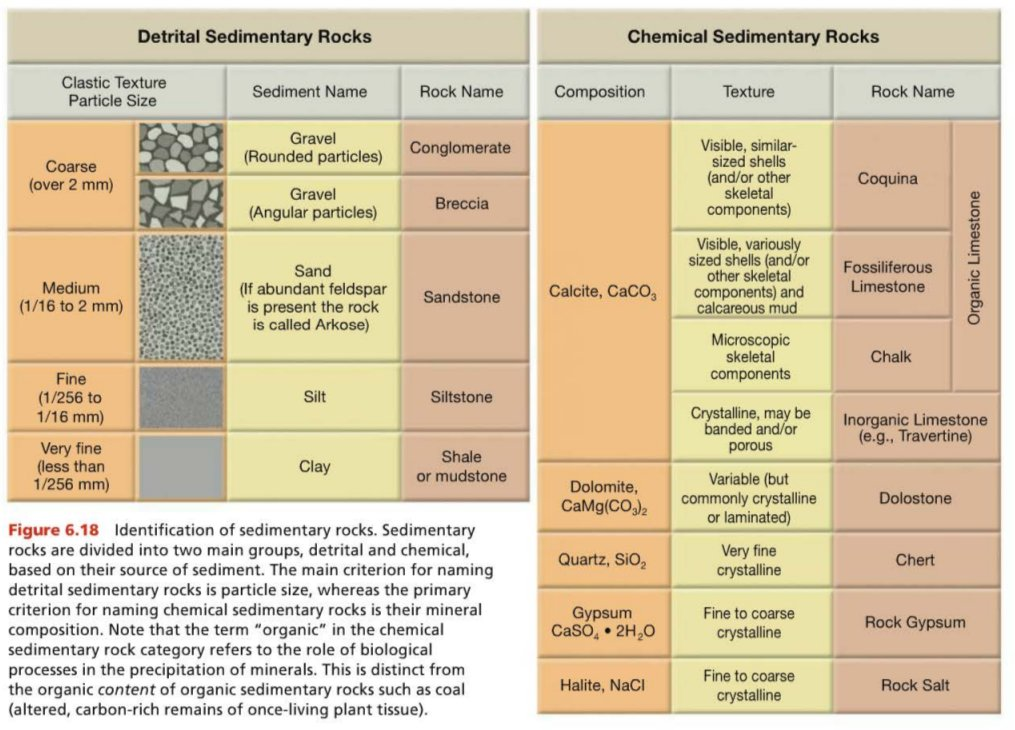
\includegraphics[width=7in]{sedimentary}

\subsection{Coal} % (fold)
\label{sub:coal}
Coal is the product of large amounts of plant material being burried for millions of years. This usually happens in a swamp since its water is oxygen deficient to prevent decay allowing the plants to be attacked by bacteria. This liberates oxygen and hydrogen from the plant material increasing the percentage of carbon. These bacteria evetually die due to lack of oxygen or acid from the plants.

At this point we have partial decomposition into a soft brown material called \textbf{peat}. With shallow burrial the peat becomes \textbf{lignite}, a soft brown coal. From there higher temperatures cause chemical reactions and yield water and organic gases, The pressure from above sediment pushes out the volitiles resulting in \textbf{bituminous}, soft black coal. Eventually metamorphism kicks in resulting in \textbf{anthracite} .
% subsection coal (end)

\subsection{Classification of Sedimentary Rocks} % (fold)
\label{sub:classification_of_sedimentary_rocks}
First we divide into detrital and chemical rocks. Detrital are then divided by particle size and chemical are divided based on composition. Texture also plays a role, though there are only to main kinds. \textbf{Clastic} rocks have discrete fragments and particles taht re cemented and compacted together and \textbf{non-clastic} rocks have a pattern of interlocking crystals.
% subsection classification_of_sedimentary_rocks (end)

\subsection{Sedimentary Stuctures} % (fold)
\label{sub:sedimentary_stuctures}
Sedimentary rocks usually form layers called \textbf{strata} of unique properties. Between each strata are \textbf{bedding planes} which are flat surfaces along which rocks separate or break. These are indicated by changes in grain size or composition of the rocks being deposited. These usually mark the end of a short-distance transport.

Usually strata are horizontal due to gravity but they ca be inclined due to \textbf{cross-bedding}, usually found in sand dunes or deltas. \textbf{Gradded beds} are when the particle type changes gradually usually due to currents rapidly slowing down (can also be caused by a storm).

You can get ripples anywhere the current often changes direction called oscilation ripples (these are symmetrical) or from  regular currents crossing sedimemt piles resulting in a gentle side facing the current and steep side away.

Storms can form \textbf{hummocky cross-stratification} where we get low angle laminations with wavelike undulations (the strata bulge and are not just flat layers).
% subsection sedimentary_stuctures (end)

\subsection{Fossils} % (fold)
\label{sub:fossils}
Fossils are very helpful in determining the age of rocks. They come in two forms, body fossils and trace fossiles. Very rarely do we get body fossils. To do so the remains must not get fucked with by other animals and microbes, usually caused by sudden entombment (like with tar or amber). The most famous example is the Burgess Shale in BC where organisms were rapidly burried by sediment at the foot of some submarine escarpment. There was little oxygen to support decomposition and the fossils were preserved carbonization (preservation as a carbon film on the loss of volitiles) and minerals precipitating on the tissue surface. Fossils can also be recorded as imprints (usually animals after the Paleozoic area that lacked exoskeletons).

We usually only get fossils of the hard parts since tissue doesn't preserve well. We can get these by \textbf{petrification} where minerals fill the pores of the remains (common for bone and wood). We can also preserve things through \textbf{replacement} where original material is replaced by another material (usually a sturdier material). Preservation can also occur by \textbf{moulding} where the surrounding material forms a mould of the fossil.

Trace fossils are not actual remains, but records of activities (like foot prints and burrows ans such).
% subsection fossils (end)
% section chapter_6_sedimentary_rocks (end)

\section{Chapter 7: Metamorphic Rock} % (fold)
\label{sec:chapter_7_metamorphic_rock}
\subsection{Metamorphism} % (fold)
\label{sub:metamorphism}
This is the changes that take place when a rock is subjected to temperatures or pressures markedly different from those in which it originally formed.
% subsection metamorphism (end)

\subsection{Controlling Factors in Metamorphism} % (fold)
\label{sub:controlling_factors_in_metamorphism}
The composition of a metamorphic rock usually mimics that of its parent rock, but its texture and specific mineral makeup are determined by the process applied to it.

\subsubsection{Heat as a Metamorphic Agent} % (fold)
\label{sub:heat_as_a_metamorphic_agent}
The primary role of heat in metamorphism is to change the chemical characteristics of rocks. Heat is what drives that basic chemical reactions that cause metamorphism and creates mobility  and reactivity. Heat is first given off by an intrusive igneous body, or it can be given off by the earth's internal heat it the rocks are buried far enough. Different minerals metamorphose at different temperatures.
% subsection heat_as_a_metamorphic_agent (end)

\subsubsection{Pressure as a Metamorphic Agent} % (fold)
\label{sub:pressure_as_a_metamorphic_agent}
The primary role of pressure in metamorphism is to change the physical properties of rocks. Pressure can influence heat so it does have a secondary role in determining the distribution of elements in rocks.

\paragraph{Confining pressure} % (fold)
\label{par:confining_pressure}
This is another name for uniform stress in which pressure is applied from all directions to squish the rock to its smallest possible volume. With this kind of pressure no deformation occurs.
% paragraph confining_pressure (end)

\paragraph{Directed Pressure} % (fold)
\label{par:directed_pressure}
Also known as differential pressure, this is the unequal applicaiton of pressure which causes deformation, usually associated with tectonic activity. One type is \textbf{compressional stress} where the tectonic plate ``shortens'' resulting in rocks pushing together. A second type is \textbf{tensional stress} when a tectonic plate ``lengthens'' causing rocks to pull apart. The final type is \textbf{shear stress} where forces are parallel but opposite.

At places of low temperature rocks are brittle and tent to fracture under directed pressure. Higher temperature rocks are more malleable and deform under pressure causing their grains to flatten and elongate in the direction of least pressure. This effects the texture of the rocks. We call the layered texture that results \textbf{foliation}.
% paragraph directed_pressure (end)
\paragraph{Foliation} % (fold)
\label{par:foliation}
Foliation development is influenced by the rotation of grains, the changing shape of grains, and the recrystallization of minerals to form new grains. The rotation of grains only dominates in environments of low stress as it is a simple change that requires less force. Recrystallization happens when components are dissolved and transported to be reprecipitated on other grains. It usually flows from high stress zones to areas of less stress.
% paragraph foliation (end)
% subsection pressure_as_a_metamorphic_agent (end)

\subsubsection{Chemically Active Fluids} % (fold)
\label{sub:chemically_active_fluids}
When magma cools it releases hot water into the surrounding rocks. Similarly rocks can contain water as they sink down and start to metamorphose releasing hot water into the area. Both of these conditions result in chemically active fluids at the sight of metamorphism which can carry ions from one site to another facilitating recrystallization. When the rocks surrounding a pluton are of different composition to the fluids being released there will be an exchange causing the host rock to have a different chemical composition in a process called \textbf{metasomatism}.
% subsection chemically_active_fluids (end)

% subsection controlling_factors_in_metamorphism (end)

\subsection{Metamorphic Grade and Index Minerals} % (fold)
\label{sub:metamorphic_grade_and_index_minerals}
\textbf{Metamorphic grade} is the intensity of metamorphism the rock has experienced. This is indicated by the sequential appearence of minerals due to different specific temperatures. We use some minerals as a \textbf{index materials} to evaluate against when determining the grade of metamorphic rock. Rocks that contain low grade minerals (ones that form at low temperatures) are low grade rocks. If a rock is heated without directed pressure being applied we have only the index materials to indicated metamorphic grade, otherwise we can use grain size and orientation to evaluate the rock.
% subsection metamorphic_grade_and_index_minerals (end)

\subsection{Burial Metamorphism} % (fold)
\label{sub:burial_metamorphism}
\textbf{Burial Metamorphism} is the mild alteration of a rock by an increase in temperature and pressure due to being buried. Its basically one step past sediment diagenesis. Here geothermal heat is enough to recrystallize some minerals to form low grade metamorphic rock.
% subsection burial_metamorphism (end)

\subsection{Contact Metamorphism} % (fold)
\label{sub:contact_metamorphism}
\textbf{Contact Metamorphism} is when ricks immediately surrounding an igneous body are cooked and altered. These define a zone of altered rock called \textbf{aureole}. These rocks tend to not be foliated as no pressure has been applied. This results in random crystal orientation. In the case of large grains we get a spotted appearance called \textbf{porphyroblastic texture}. As rocks get farther from the pluton their grade decreases.
% subsection contact_metamorphism (end)

\subsection{Regional Metamorphism} % (fold)
\label{sub:regional_metamorphism}
Most metamorphic rocks are created by \textbf{regional metamorphism} which is metamorphism over a wide area due to pressures and temperatures at convergent plate boundaries. Here there is substantial confining pressure causing deformation. The section pushed down at the boundary sufferes the most heat and pressure causing intese metamorphism. This means that the cores of most mountains are metamorphic rock.
% subsection regional_metamorphism (end)

\subsubsection{Regional Metamorphism and Shale} % (fold)
\label{sub:regional_metamorphism_and_shale}
Metamorphism is the process that turns shale into slate, phyllite, shist, and gneiss.

\paragraph{Slate} % (fold)
\label{par:slate}
This is a fine grained folliated rock composed of mica flakes produced by low grade metamorphism. You can tell it apart from shale because it doesnt have a earthy smell and rings when you flick it. Slate has very distinct \textbf{rock cleavage} (not the same as mineral cleavage or bedding).
% paragraph slate (end)

\paragraph{Phyllite} % (fold)
\label{par:phyllite}
This is produced at slightly higher temperatures and pressures than slate. It also has rock cleavage, but is a wavy appearance rather than the straight lines of slate due to higher directed pressure on it.
% paragraph phyllite (end)

\paragraph{Schist} % (fold)
\label{par:schist}
This has medium grains and is dominated by platy mica large enough to be see without aid. They have a distinctive foliation called \textbf{schistosity} that we use to define them.
% paragraph schist (end)

\paragraph{Gneiss} % (fold)
\label{par:gneiss}
These are medium grain rocks dominated by elongate minerals of high metamorphic grade. The high metamorphism separates the light and dark components into layers giving it a stripy appearance called \textbf{gneissic texture}. It will often break along layers of platy minerals.
% paragraph gneiss (end)
% subsection regional_metamorphism_and_shale (end)

\subsubsection{Regional Metamorphism and Basalt} % (fold)
\label{sub:regional_metamorphism_and_basalt}
Basalt based rocks have a ahigher abudance of minerals with iron and magnesium than shale based rocks resulting in much less foliation. Instead of platy minerals it is dominated by elongated minerals which produce less pronounced foliation.

\paragraph{Greenschist} % (fold)
\label{par:greenschist}
At low grades of metamorphism feromagnesian minerals are hydrated to form different minerals like chlorite that provide foliation and a green color to the rock. Greenschist is equivalent to slate and phyllite.
% paragraph greenschist (end)

\paragraph{Amphibolite} % (fold)
\label{par:amphibolite}
At higher temperatures and pressures hydrated minerals lose water and are converted to amphiboles forming the rock called amphibolite. It is equivalent grade to schist. Amphibole crystals are very thin and needle-like resulting in a defined orientation taht produces less distinct foliation than greenschist.
% paragraph amphibolite (end)

\paragraph{Granulite} % (fold)
\label{par:granulite}
At higher temperatures and pressures the amphibolite is dehydrated more to produce proxenes and garnets in a rock called granulite. It is equivalent grade to gneiss. The crystals in this type of rock are block shaped and coarse grained resulting in little elongation and little orientation.
% paragraph granulite (end)

% subsection regional_metamorphism_and_basalt (end)

\subsubsection{Upper Limit of Regional Metamorphism} % (fold)
\label{sub:upper_limit_of_regional_metamorphism}
At the most extreme environments rocks begin to partially melt and start trasnforming into igneous rocks. The ambigous state in between has rocks called \textbf{migmatites} and have parts that are metamorphic and parts that are igneous. The lighter rocks tend to have the lowest melting temperatures resulting in them making up igneous bands while the darker minerals make up the metaphoric bands.
% subsection upper_limit_of_regional_metamorphism (end)

\subsubsection{Regional Metamorphism and Nonfoliated Rocks} % (fold)
\label{sub:regional_metamorphism_and_nonfoliated_rocks}
Sometimes the parent rock lacks the necessary elements to produce the platy or elongate mineral grains to create foliation in metamorphic rocks. In cases of pure quartzite or marbles (rocks made of quartz an calcite only) the metamorphic rocks formed from contact and regional metamorphism can look identical.
% subsection regional_metamorphism_and_nonfoliated_rocks (end)
\subsection{Subduction Zone Metamorphism} % (fold)
\label{sub:subduction_zone_metamorphism}
\textbf{Subduction zone metamorphism} is a specific form of regional metamorphism that takes place in the region of a subducted slab. These are characterized by high pressure and low temperatures. In this environment a blue sodium rich amphibole forms called glaucophane. The rock that forms from this has foliation and is called \textbf{blueshist}. Further subduction pulls rocks into the mantle where it is transformed into \textbf{eclogite}.
% subsection subduction_zone_metamorphism (end)

\subsection{Metamorphic Facies and Plate Tectonics} % (fold)
\label{sub:metamorphic_facies_and_plate_tectonics}
\textbf{Metamorphic facies} are defined by a distinctive assemblage of minerals used to designate a particular set of metamorphis environmental conditions recorded in rocks. This allows us to interpret rocks created by different types of metamorphism in a single context. The names of metamorphic facies refer to the basaltic parent rocks. Basically these are sections of a temperature by pressure graph that we label as resulting in similar rocks.
% subsection metamorphic_facies_and_plate_tectonics (end)

\subsection{Ancient Metamorphic Environments} % (fold)
\label{sub:ancient_metamorphic_environments}
The oldest known rocks are found in large expanses of metamorphic rocks called \textbf{sheilds}. Great Bear Lake in Canada has the oldest known rocks at 4.03 billion years old. Shields are made up of rocks that resemble the cores of young mountains leading geologists to believe they are the remains of super old mountains that got weathered down to nothing.
% subsection ancient_metamorphic_environments (end)

% section chapter_7_metamorphic_rock (end)


\section{Chapter 8: Geologic Time} % (fold)
\label{sec:chapter_8_geologic_time}
\subsection{Relative Dating} % (fold)
\label{sub:relative_dating}
\subsubsection{Geologic Time} % (fold)
\label{subsub:geologic_time}
\textbf{Relative Dating} is the notion that rocks are placed in their sequence of formation, It gives us the temporal order of events with no hard numbers associated.
% subsection geologic_time (end)

\subsubsection{Law of Superposition} % (fold)
\label{sub:law_of_superposition}
\textbf{Nicolaus Steno} first recognized a sequence of historical events in an outcrop of sedimentary rock and cam up with \textbf{the law of superposition} which states that in sedimentary rocks that have not been deformed a bed is older the than the one above it.
% subsection law_of_superposition (end)

\subsubsection{Principle of Original Horizontality} % (fold)
\label{sub:principle_of_original_horizontality}
The \textbf{principle of original horizontality} is also credited to Steno and states that layers of sediment are generally deposited in horizontal layers. This means that if we see a flat horizontal layer it has not been disturbed from its original shape.
% subsection principle_of_original_horizontality (end)

\subsubsection{Principle of Cross Cutting Relations} % (fold)
\label{sub:principle_of_cross_cutting_relations}
The \textbf{principle of cross-cutting relations} states that when something cuts through layers(like a fault of intrusion) then we can assume that it is younger than the layers it is cutting through. A layer wouldn't form around a gap.
% subsection principle_of_cross_cutting_relations (end)

\subsubsection{Inclusion} % (fold)
\label{sub:inclusion}
\textbf{Inclusions} are fragments of one rock that trapped within another. We can say that the rock mass adjacent to the rock with the inclusion must have been there first inorder to donate the rock that ended up included.
% subsection inclusion (end)

\subsubsection{Unconformities} % (fold)
\label{sub:unconformities}
An \textbf{unconformity} is a gap in the record where depositing of sediment was interrupted or eroded away. These often represent significant events. There are three types.

\paragraph{Angular Unconformity} % (fold)
\label{par:angular_unconformity}
This is the tilted or folded sedimentary rocks that are overlain by younger flat layers. It indicates a time between deposition where deformation occurred to tilt the current layers to a new angle.
% paragraph angular_unconformity (end)

\paragraph{Disconformity} % (fold)
\label{par:disconformity}
These are very hard to identify because the layers on either side of them are parallel and normal. Basically they are just gaps between layers that are not perfectly flat.
% paragraph disconformity (end)

\paragraph{Nonconformity} % (fold)
\label{par:nonconformity}
This is where the break separates much older rock from much younger rock. They are formed when periods of uplift or erosion bring deep rocks to the surface where younger layers can be built on them.
% paragraph nonconformity (end)

% subsection unconformities (end)

% subsection geologic_time_scale (end)
\subsection{Correlation of Rock Layers} % (fold)
\label{sub:correlation_of_rock_layers}
\textbf{Correlation} is that task of matching up rocks of similar age in different regions to develop a geologic time scale.

\subsubsection{Correlation by Physical Criteria} % (fold)
\label{sub:correlation_by_physical_criteria}
When outcrops are near to each other we can not the position of a layer and correlate that layer to the one in the same position the near by outcrop. When the entire sequence is not visible we use the physical characteristics of the rock to find which layer matches it. This process doesn't work over large distances.
% subsection correlation_by_physical_criteria (end)

\subsubsection{Fossils and Correlation} % (fold)
\label{sub:fossils_and_correlation}
We can know that layers that contain the same types of fossils must have formed within the lifetime of that species. This was discovered by \textbf{William Smith}. Further more we know that fossil organisms succeed each other allowing us to form a time line of fossils and corresponding layers. Fossils that are particularly widespread and thus more useful for correlation are called \textbf{index fossils}. If a index fossil is not present we can use a collection of fossils to find the overlapping time frame of the layer.

Fossils can also be used to give hints to the kind of environment in the area at the time they died and that layer was formed.
% subsection fossils_and_correlation (end)
% subsection correlation_of_rock_layers (end)


% subsection relative_dating (end)

\subsection{Dating with Radioactivity} % (fold)
\label{sub:dating_with_radioactivity}
This is the process by which we give dates numbers.

\subsubsection{Radioactivity} % (fold)
\label{sub:radioactivity}
An unstable ``parent'' isotope decays into a more stable ``daughter'' isotope. By knowing the process and time this takes we can calculate dates for stuff. Decay rates can be precisely calculated and are unaffected by conditions deep in earth. We use the rate of decay with the amount of daughter isotope to calculate when the radioactive parent was first incorporated to that mineral.
% subsection radioactivity (end)

\subsubsection{Half Life} % (fold)
\label{sub:half_life}
The half life of a mineral is the time required for a sample to decay to half its mass (parent to daughter mass ratio of 1:1).
% subsection half_life (end)

\subsubsection{Radiometric Dating} % (fold)
\label{sub:radiometric_dating}
In this version of dating we calculate based on the mass of daughter isotope only since we know that at the start of the clock (first crystalization of the rock) there was no daughter isotope present. Error can be introduced if anything influenced the amount of parent or daughter isotopes anywhere in the life time of the rock.

A common method is looking at the amount of argon-40 produced by the decay of potassium-40 since potassium is abundant and has only one common radio active isotope. Argon is unfortunatly a gas which means that some of the daughter isotope can escape and skew the radiometric date. To avoid this and other problems like it geologists use fresh unweathered rock when dating things.
% subsection radiometric_dating (end)

\subsubsection{Dating with Carbon-14} % (fold)
\label{sub:dating_with_carbo_14}
Carbon-14 is used for \textbf{radiocarbon dating} since it has a much shorter half life (it can only be used for events <50 000 years ago). All organisms absorb carbon-14 as it is mixed into carbon dioxide (forms when cosmic ray bombardment warps carbon in carbon dioxide). While an organism is alive the decaying carbon-14 is replaced keeping it proportion constant, but when it dies it stops absorbing c14 allowing decay to begin.
% subsection dating_with_carbo_14 (end)
% subsection dating_with_radioactivity (end)


\subsection{Geologic Time Scale} % (fold)
\label{sub:geologic_time_scale}
The \textbf{geologic time scale} is the scale of time created in the nineteenth century using relative dating.

\subsubsection{Structure of the Time Scale} % (fold)
\label{sub:structure_of_the_time_scale}
The largest unit in the scale is eons, then eras, then periods, and finaly epochs.

List of eons and eras
\begin{itemize}
    \item Cambrian/Phanerozoic - rocks containd abundant fossils
    \begin{itemize}
        \item paleozoic - ancient life
        \item mesozoic - middle life
        \item cenozoic - resent life
    \end{itemize}
    \item precambrian - time between birth of planet and first life
    \begin{itemize}
        \item hadean
        \item archean
        \item proteozoic
    \end{itemize}
\end{itemize}
% subsection structure_of_the_time_scale (end)

\subsection{Difficulties Dating the Geologic Time Scale} % (fold)
\label{sub:difficulties_dating_the_geologic_time_scale}
Radio metric dating begins when a mineral crystalizes which can lead to problems when different minerals crystalize at different times. Even worse is that the grains may not be the same age as the rock in which they occur. We attempt to date sedimentary rocks by relating strata to igneous masses.
% subsection difficulties_dating_the_geologic_time_scale (end)








% section chapter_8_geologic_time (end)

\end{document}
